% ACL-style draft — compile with: tectonic main.tex (bibtex pass handled by latexmk-like reruns; see README)
\documentclass[11pt]{article}
\usepackage[review]{acl}
\usepackage{times}
\usepackage{latexsym}
\usepackage[T1]{fontenc}
\usepackage[utf8]{inputenc}
\usepackage{microtype}
\usepackage{inconsolata}
\usepackage{graphicx}
\usepackage{booktabs}
\usepackage{amsmath}

\title{Learning to Apply, Not to Memorize: \\ Policy-in-Context Fine-Tuning Generalizes to Unseen Organizational Policies}

\author{Anonymous \\ \texttt{draft v0.6 --- not for distribution}}

\begin{document}
\maketitle

\begin{abstract}
The people who own a task in an organization are rarely programmers or model experts, and the documents that govern their work---policies, runbooks, checklists---change on the organization's schedule. We build on a simple workflow: a worker first solves the job in conversation with an agent; the recorded sessions are expressed in the declarative work language OpenWorkLang and compiled by OpenWorkCompiler, so that policies become an ontology with rules, calculations become programs, and judgment goes to a small local model. This paper tests the doubtful link in that chain: can a small model learn the \textbf{skill} of judgment---applying whatever policy it is given in context — rather than memorizing any particular policy? On 34 organizational decision cases (3,400 decisions labeled by a deterministic rules engine), a QLoRA-tuned 7B model reaches \textbf{72.9\%} exact match (verdict, routing, parameters, and a \emph{correct} cited rule) on policies never seen in training, evaluated leave-case-out so every policy is unseen exactly once (cluster-bootstrap 95\% CI $[64.7, 80.9]$), versus 15.0\% for the untrained model under identical serving. Controls pin down what was learned: \textbf{88.0\%} on counterfactual policies where prior knowledge scores zero by construction, 50.0\% for a 3-shot in-context-learning baseline, $\pm$4.8pp variance across training seeds. A negative control bounds the recipe: the same recipe on byte-exact arithmetic scores 0/6---with chain-of-thought targets, and even for a tool-less frontier model---so calculation is compiled to code once rather than delegated to an LLM on every run. Because compilation starts from a work session the organization already paid for, the frontier-token break-even is the \textbf{second run}.
\end{abstract}

\section{Introduction}

In most organizations, correct behavior is defined by \emph{documents}---decision policies, support runbooks, escalation matrices, grading rubrics, editorial style guides, compliance checklists---and those documents change on the organization's schedule, not the model's. Any AI system built on them needs a particular decomposition: the \textbf{content} (what the document says today) must live \emph{in context}, where it can be swapped the day it changes, while the \textbf{skill} (how to read such a document and apply it faithfully to a case) can live \emph{in weights}. This paper measures whether that skill is actually learnable by supervised fine-tuning of a small model---and whether it transfers to documents the model has never seen.

In practice the decomposition plays out like this. The people who own these tasks are not programmers or model experts. At first they simply do their job---quotes, refund approvals, incident triage---in conversation with an agent. Those working sessions already contain the job's policies, its calculations, and its way of judging. Expressed in a declarative work language (OpenWorkLang) and run through its compiler (OpenWorkCompiler), the policies become an ontology with rules, the calculations become programs, and the judgment goes to a trained small model---yielding a task-specific execution-and-decision tool that runs on a local GPU, without a frontier LLM, at a fraction of the tokens. This paper puts the most doubtful link of that chain to the test---is judgment actually learnable by a small model?---and backs the other links with controls and measurements (calculation belongs to programs, \S\ref{sec:control}; the token economics, \S\ref{sec:economics}).

We study the cleanest instance of this class that still admits a deterministic grader: organizational decision policies. When an employee asks ``can I give this customer a 12\% discount?'', the organization does not want an oracle's opinion. It wants \emph{its own policy applied}: the ordered rules checked top-down, the first matching rule cited, the case routed to the approver the policy names, and the band the policy deliberately left open (``5--10\%: AI may recommend, team lead approves'')---and only that band---filled by a recommendation. Three properties shape the ML problem, each instantiating the general decomposition:

\begin{enumerate}
  \item \textbf{The documents change faster than models.} A model that memorized policy $P$ is wrong the day $P$ becomes $P'$. The content must live \emph{outside} the weights.
  \item \textbf{Judgments must be auditable.} ``Approve'' is not an answer; ``approve, route to director, citing \texttt{strategic\_retention\_band} whose condition holds on this record'' is.
  \item \textbf{Discretion is declared, not inferred.} The document says where the model may recommend; confidence thresholds do not.
\end{enumerate}

Prior work internalizes policies into weights \citep{trimpi2025}, benchmarks agents given domain policy guidelines \citep{taubench2024,rulearena2024}, or measures robustness to rule updates \citep{guidebench2025}. What is missing is the combination deployment actually needs: \textbf{fine-tune a small, locally servable model on the \emph{transferable skill} of applying an arbitrary in-context policy, and measure transfer to policies never seen in training.}

Declarative decision policies make the skill (ordered evaluation, first-match, grounded citation) non-trivial while keeping correctness checkable to the byte. Whether the recipe transfers to messier members of the document class is an open question we scope explicitly, with a roadmap, in \S\ref{sec:discussion}.

Our contributions:
\begin{itemize}
  \item \textbf{Task \& corpus} (\S\ref{sec:task}): 34 decision cases across 10 organizational functions, each declared as an ontology plus ordered rules with explicit discretion bands, compiled by a deterministic engine into 3{,}400 labeled decisions with cited rules and grounded conditions.
  \item \textbf{A strict deterministic grader} (\S\ref{sec:grading}): exact match on verdict, route, parameters \emph{and} cited rule, plus a check that the cited rule's condition actually holds on the record.
  \item \textbf{The transfer result} (\S\ref{sec:transfer}): leave-case-out over all 34 policies, 72.9\% exact $[64.7, 80.9]$ vs.\ 15.0\% raw under identical bf16 greedy serving; ICL ladder $15.0 \rightarrow 50.0 \rightarrow 72.9$.
  \item \textbf{The counterfactual control} (\S\ref{sec:counterfactual}): 88.0\% on flipped policies where priors score zero by construction.
  \item \textbf{Negative control and placement economics} (\S\ref{sec:control}--\ref{sec:economics}): the same recipe on byte-exact arithmetic fails (0/6), survives a CoT-target ablation, and is matched by a tool-less frontier model failing the same gate---justifying compilation to code over per-run tool calls, with a measured second-run break-even.
\end{itemize}

\section{Related Work}

\paragraph{Policy internalization vs.\ policy-in-context.} Multimodal Policy Internalization \citep{trimpi2025} trains policies \emph{into} model parameters so the policy need not be in context at inference---the opposite maintenance bet from ours. Its ``Policy Override'' setting supplies an updated policy in context at inference as a \emph{generalization probe} of the internalized model; we make in-context application the training objective itself. Policy Reasoning Traces \citep{prt2025} improves compliance assessment on specific policies such as HIPAA and GDPR with per-policy instance-level train/test splits; cross-policy transfer appears only as an auxiliary analysis, not as the held-out-policy protocol we use. GuideBench \citep{guidebench2025} benchmarks robustness to rule updates.

\paragraph{Policy-following benchmarks.} $\tau$-bench \citep{taubench2024} evaluates state-of-the-art agents given domain policy guidelines; RuleArena's \citep{rulearena2024} findings distinguish failures of rule identification from failures of the computations the rules require---directly anticipating our \S\ref{sec:control}; CRMArena-Pro \citep{crmarena2025} assesses agents across enterprise scenarios. A contemporaneous enterprise benchmark \citep{enterprisebench2026} independently builds rule-engine-judged decisions; it is evaluation-only and has no discretion bands. DMN \citep{dmn2024} has long standardized ordered decision rules with FIRST-hit semantics; our DSL is deliberately in that family---the ML contribution is the transfer measurement, not the rule language.

\paragraph{SFT and arithmetic.} Faith and Fate \citep{faithfate2023} shows Transformers fail at compositional multi-step arithmetic; \citet{sftmemorizes2025} shows SFT tends to memorize and struggles out-of-distribution; PAL \citep{pal2022} offloads the solution step to a Python interpreter. Our contribution is the \emph{pairing}: the same recipe, corpus scale and gate that fail on arithmetic succeed on rule application---and a tool-less frontier model fails the same arithmetic gate, sharpening ``small models can't compute'' into ``inference can't compute.''

\paragraph{Small-model deployment.} \citet{slmposition2025} argue small models are the future of agentic AI and outline an LLM-to-SLM conversion algorithm; we supply a trained-skill recipe and transfer measurement for one high-value slot (policy application) and a deterministic gate that even frontier models fail for another (derivation), yielding a placement rule rather than a preference.

\section{Task and Corpus}\label{sec:task}

\subsection{Decision cases}
A \emph{case} declares one recurring organizational decision: the deciding role, an \textbf{ontology} (entities, attributes, relations), a feature space, \textbf{ordered rules} (\texttt{when} condition $\rightarrow$ verdict, route, parameters, rationale), optional \textbf{discretion bands} (\texttt{defer: slm\_recommend} with the band's limits as parameters), and a fallback. The corpus holds \textbf{34 cases across 10 functions} (sales, finance, support, HR, procurement, legal, IT operations, marketing, logistics, security). A deterministic engine samples records from each case's feature space and applies first-match semantics to produce \textbf{100 labeled decisions per case} (3{,}400 total), each with the applied rule's name, its condition, and a rationale. Generation is seeded and byte-reproducible.

\subsection{Policy-in-context format}
Per instance the model receives: a system turn naming the organization, role and decision; the case's ontology and its \emph{full ordered rule list} (YAML, verbatim); and the record. It must output one JSON object \texttt{\{verdict, route, params, cited\_rule, rationale\}}. Nothing about any specific policy is in the weights; a rule edit changes behavior with no retraining.

\subsection{Grading}\label{sec:grading}
An answer is \textbf{exact} iff verdict, route and parameters equal the engine's decision \emph{and} the cited rule is the first-matching rule \emph{and} that rule's condition actually holds on the record (the last check fails fabricated grounds even when the verdict is guessed right). A \textbf{relaxed} variant accepts a cited rule that is not first-match but whose condition genuinely holds with all other fields correct. We also report verdict-only accuracy. Because held-out items cluster by policy, all confidence intervals are \textbf{case-cluster bootstrap} (10{,}000 resamples over cases).

\subsection{Honest scope}\label{sec:scope}
The corpus is synthetic and self-graded: the engine that labels is the engine that grades, the policies are already machine-readable, and rule-condition field names match record keys---the entity-alignment difficulty of prose policies is absent, as are noisy fields and annotator disagreement. We claim transfer of \emph{policy application on declarative policies}, a deliberately clean substrate; \S\ref{sec:discussion} discusses the path to prose policies.

\section{Experimental Setup}

\paragraph{Model \& training.} Qwen2.5-7B-Instruct, QLoRA ($r{=}16$, $\alpha{=}32$, dropout 0.05, all linear projections), completion-only loss, 2 epochs, LR $10^{-4}$ cosine, bf16 compute on one RTX 4090 ($\approx$12 min/run). Training data: 28 cases $\times$ 40 instances (1{,}120 rows); 6 cases held out \emph{entirely}. The environment is pinned and every run writes a manifest (seed, epochs, data and adapter SHA-256, package versions).

\paragraph{Serving \& fairness.} All models---tuned \emph{and} raw baselines---are evaluated through the same bf16 server with greedy decoding. (Re-running raw baselines under identical serving moved raw 7B from 16.7\% to 15.0\%; the quantization confound does not explain the gap.)

\paragraph{Splits.} (a) \emph{Pinned}: 6 held-out cases $\times$ 10 instances, plus 56 seen-policy/unseen-instance items. (b) \emph{Leave-case-out (LOCO)}: 6 folds re-trained with the same recipe so every one of the 34 policies is unseen exactly once (340 items, 34 clusters).

\section{Results}

\subsection{Transfer to unseen policies}\label{sec:transfer}

\begin{figure*}[t]
  \centering
  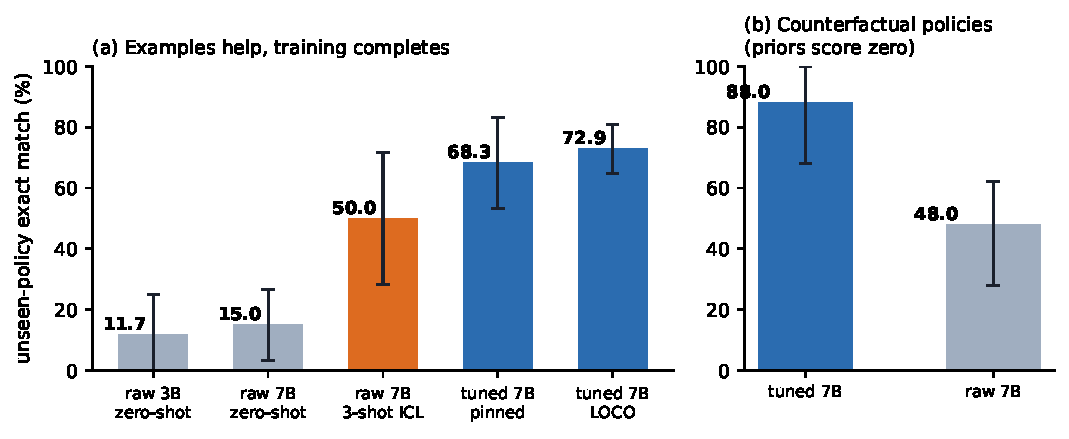
\includegraphics[width=0.98\textwidth]{../figs/fig1_ladder_counterfactual.pdf}
  \caption{(a) Unseen-policy exact match with case-cluster bootstrap 95\% CIs. (b) The counterfactual control: on records where the flipped policy decides differently, priors score zero by construction.}
  \label{fig:ladder}
\end{figure*}

\begin{table}[t]\small
  \centering
  \begin{tabular}{@{}lrr@{}}
    \toprule
    model (identical serving) & exact & 95\% CI \\
    \midrule
    raw 3B, zero-shot        & 11.7\% & $[0.0, 25.0]$ \\
    raw 7B, zero-shot        & 15.0\% & $[3.3, 26.7]$ \\
    raw 7B, 3-shot ICL       & 50.0\% & $[28.3, 71.7]$ \\
    tuned 7B (pinned split)  & 68.3\% & $[53.3, 83.3]$ \\
    \textbf{tuned 7B (LOCO)} & \textbf{72.9\%} & $\mathbf{[64.7, 80.9]}$ \\
    \bottomrule
  \end{tabular}
  \caption{Unseen-policy exact match. LOCO holds every one of the 34 policies out exactly once.}
  \label{tab:main}
\end{table}

LOCO fold accuracies range 65.0--80.0\%: the pinned-split result is not an artifact of one partition (Table~\ref{tab:main}, Figure~\ref{fig:ladder}a). Across 3 training seeds, unseen exact is $62.8\% \pm 4.8$pp---run variance is real and reported; no seed approaches the raw baseline. In-context examples help substantially ($15 \rightarrow 50\%$) but fine-tuning adds ${\sim}20$pp over ICL while removing per-request example tokens. Per-policy scores range 1/10--10/10 under LOCO (Figure~\ref{fig:perpolicy}); policies whose conditions embed date/limit arithmetic (leave, overtime, payment extension) sit at the bottom, foreshadowing \S\ref{sec:control}.

\begin{figure}[t]
  \centering
  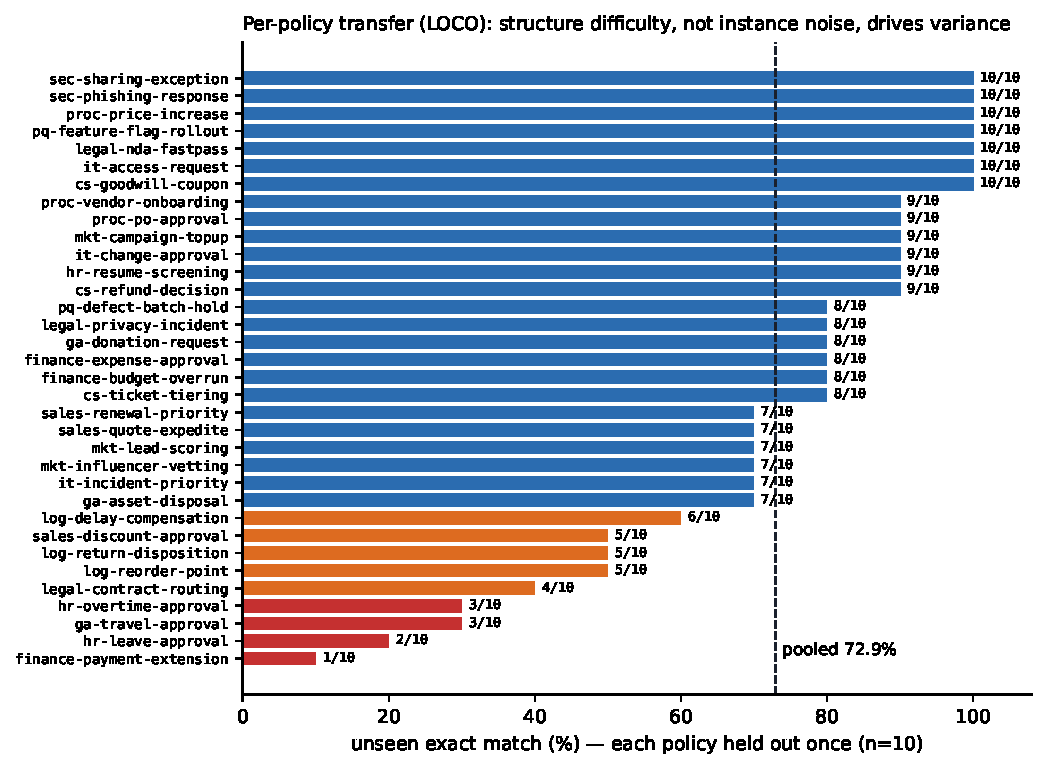
\includegraphics[width=\columnwidth]{../figs/fig2_per_policy.pdf}
  \caption{Per-policy transfer under LOCO; every policy is unseen exactly once ($n{=}10$ each).}
  \label{fig:perpolicy}
\end{figure}

\subsection{What was learned: the counterfactual control}\label{sec:counterfactual}
We flip approve$\leftrightarrow$reject in every rule (and the fallback) of the held-out cases and evaluate \textbf{only on records where the flipped policy decides differently from the original}---on this subset, answering from priors or from the original policy scores zero by construction. The tuned model scores \textbf{88.0\%} (44/50); raw 7B scores 48.0\% (Figure~\ref{fig:ladder}b). Combined with \S\ref{sec:transfer}, this is direct evidence that fine-tuning taught \emph{application of the in-context policy}, not policy content and not world priors.

\subsection{Negative control: the same recipe cannot learn computation}\label{sec:control}
We ran the identical recipe (same trainer, gate, corpus scale: 300 examples) on a \emph{derivation} task from the same product family: regenerate a customer's renewal-pricing files (22 numeric fields) byte-exactly for held-out customers, judged by a deterministic gate.

\begin{table}[t]\small
  \centering
  \begin{tabular}{@{}lrr@{}}
    \toprule
    arm & gate & field acc. \\
    \midrule
    SFT 7B (plain targets)     & 0/6 & --- \\
    SFT 7B (CoT targets)       & 0/6 & 86.4\% \\
    frontier, same prompt, no tools & 0/6 & 93.6\% \\
    \bottomrule
  \end{tabular}
  \caption{The arithmetic negative control. Both tuned and frontier arms fail almost solely on two long-division fields.}
  \label{tab:control}
\end{table}

This is a \emph{control, not a discovery}---routing arithmetic to tools is settled practice. Its role: (i) it closes the ``train harder'' objection (the CoT-target ablation still fails; the frontier fails the same gate on the same two long-division fields while getting every band and discount rule right; the recorded agent originally passed because it computed with tools); (ii) field-level scores show what the exact gate hides---inference gets 20--21 of 22 fields, failing precisely where computation, not rule-reading, is required; (iii) it motivates going beyond the standard remedy: a per-run \textbf{tool call keeps the LLM in the loop on every execution} (re-deciding which tool to invoke, nondeterministically, with orchestration tokens), whereas compiling the step to the \textbf{code tier makes that decision once}, at compile time. The placement rule: derivations $\rightarrow$ code; policy judgments $\rightarrow$ trained SLM behind the deterministic gate; declared discretion bands $\rightarrow$ recommendation + human approver.

\subsection{Placement economics: break-even at the second run}\label{sec:economics}
Measured on the renewal pipeline in unique tokens (not double-counting the cumulative context an agent resends each turn): the recorded agent session costs 23{,}614 frontier tokens per run; after compilation and SLM promotion a run consumes \textbf{0 frontier tokens} (4{,}208 tokens on a local model at \$0 marginal cost, 7.4$\times$ faster, outputs reproduced 7/7 under a deterministic benchmark). Because the compiler's input is a work session the organization had to run once anyway, the frontier-token \textbf{break-even is the second run}---compared with the ${\approx}17$-transaction break-even reported for optimization-heavy compilation \citep{compiledai2026}, where the compiler spends LLM tokens searching. Escalations for genuinely new parameter values each cost one frontier call, are cached with upstream-output fingerprints, and amortize to zero on repeats. The hidden denominator is the human cost of declaring the ontology and policy; the pipeline pays off in proportion to a decision's repetition frequency---exactly the regime organizations automate first.

\section{Discussion}\label{sec:discussion}

\paragraph{Why not internalize?} A weights-internalized policy answers fast but ages instantly and cannot explain a rule edit. Policy-in-context inverts the maintenance economics: the policy file is the deployment artifact; retraining is only needed when the \emph{skill}, not the policy, drifts.

\paragraph{Beyond policy decisions.} Nothing in the recipe is specific to approval workflows: training rows are (document, record, grounded structured answer) triples, and the counterfactual control generalizes to any document class whose semantics can be programmatically perturbed. Runbooks and rubrics are the nearest neighbors; each needs its own deterministic grader, which is the actual bottleneck for widening the claim (Table~\ref{tab:roadmap}). This paper is also one tier of a larger compiled-pipeline system---recorded agent sessions lowered to code/rule/cache tiers, with the trained-SLM tier occupying the judgment slot behind a promotion gate---whose end-to-end economics (\S\ref{sec:economics}) motivate but do not depend on the transfer result.

\begin{table}[t]\footnotesize
  \centering
  \begin{tabular}{@{}p{2.1cm}p{2.4cm}p{2.2cm}@{}}
    \toprule
    document class & grader needed & status \\
    \midrule
    decision policies & rules engine & \textbf{measured (this paper)} \\
    escalation matrices & table lookup & near (catalog cases) \\
    compliance checklists & per-item rules & not started \\
    grading rubrics & answer key & not started \\
    support runbooks & state machine & not started \\
    \bottomrule
  \end{tabular}
  \caption{Generalization roadmap for the content-in-context, skill-in-weights recipe: what each document class needs before its transfer can be measured.}
  \label{tab:roadmap}
\end{table}

\paragraph{Path to prose policies.} Our substrate removes entity alignment (rule field names match record keys). The natural next experiment keeps the trained applier fixed and inserts a policy-compilation step (prose $\rightarrow$ declarative rules) in front---measuring how much of the 72.9\% survives noisy compilation, and whether the counterfactual control still holds.

\section*{Limitations}
Labels and grades come from the same engine; we mitigated with the grounds-hold check, the relaxed metric, the counterfactual control and full pinning, but human-annotated decisions with inter-annotator agreement remain future work. Scale: 34 policies, one 7B base model, one language pair (Korean prompts, mixed-language fields); cluster CIs are honest about this---$[64.7, 80.9]$ is the claim, not 72.9\%. Policies are already machine-readable; prose-policy entity alignment is untested. The frontier control uses one frontier model, one prompt format, without tools by construction.

\section*{Reproducibility}
Corpus generator, trainer (pinned; per-run manifests), evaluation code, all raw results and this draft live in one repository; every table is regenerable from a seeded generator and stored model outputs.

\bibliography{refs}

\end{document}
